\documentclass{article}

\usepackage{amsmath}
\usepackage{graphicx}
\usepackage{titlesec}
\usepackage{lipsum}
\usepackage{url}
\usepackage{float}
\usepackage{fullpage}
\setkeys{Gin}{width=0.50\textwidth}

\titleformat{\section}
  {\normalfont\scshape}{\thesection}{1em}{}

\title{Report 3}
\author{Vanessa Machuca and Luis Espino}

\usepackage{Sweave}
\begin{document}
\Sconcordance{concordance:Report_4.tex:Report_4.Rnw:%
1 17 1 1 0 4 1 1 18 1 9 18 1 1 7 4 0 1 2 2 1 1 5 4 0 1 2 4 1 1 2 1 0 1 %
1 31 0 1 2 1 1 1 2 1 0 4 1 3 0 1 2 3 1 1 5 1 1 1 9 3 0 1 1 2 0 1 1 2 0 %
2 2 2 1 1 16 1 2 1 16 1 2 2 1 1 15 1 2 1 15 1 2 25 1 1 6 1 2 1 1 1 13 4 %
0 1 2 13 1 1 4 12 1}

\maketitle





\section{Task 1 - Sparse and Smooth Linear Models}

Introduction 

The data we are working with looks at student achievement in Portuguese course at two secondary education Portuguese schools. We found the data through the UCI Machine Learning Repository. The observational units for the dataset are students. The dataset includes demographic variables like student’s school name (binary), sex (binary), age (numeric), and whether the student lives in an urban or rural area. 

It also includes variables that relate to family, including family size, parents cohabitation status (living apart or together), mother and father's education (ordinal), mother and father’s job ('teacher', 'health' care related, civil 'services' (e.g. administrative or police), 'at$\_$home' or 'other'), student’s guardian (mother, father or other), and quality of family relations ($1$ being very bad to $5$ being excellent). 

School-related variables include home to school travel time (ordinal), weekly study time (ordinal), and number of past class failures (1-3 if $n<3$, 4 otherwise). For each of two courses, students were given a graded after the first and second period as well as a final grade.  
Academic routine, habits and performance were also measured. These variables included travel time from home to school (nominal), weekly study time (nominal), number of past class failures (nominal), reason to choose school (categorical), and number of absences (numeric). Additionally, educational resources were assessed through binary measurements of extra educational support, family educational support, extra paid classes within the course subject, extracurricular activities, attended nursery school, college aspiration, and home internet access.

Finally, nominal variables that measured more personal aspect of life included frequency of outings with friends, workday alcohol consumption, weekend alcohol consumption, current health status, and being in a romantic relationship (binary). 

RR and LASSO

We will now run ridge regression (RR) and LASSO on the full varaible set, using cross validation to find lambda, and compare them. First up, RR. 

\begin{Schunk}
\begin{Soutput}
[1] 0.0225702
\end{Soutput}
\end{Schunk}

We omit categorical variables, as RR does not seem to like them very much. The lambda value which yields the lowest SSE is $0.0225702$. Onward to LASSO. 

\begin{Schunk}
\begin{Soutput}
[1] 0.03125716
\end{Soutput}
\end{Schunk}

The lambda value which yields the lowest SSE is $0.03125716$. Now to compare these two models by looking at their coefficients. Previously, we looked at plots of cefficients.

MLR 

\begin{Schunk}
\begin{Sinput}
> fwdselec <- lm(G3 ~ failures + school + sex + higher + health + Mjob, data=student_por_n)
> summary(fwdselec)
\end{Sinput}
\begin{Soutput}
Call:
lm(formula = G3 ~ failures + school + sex + higher + health + 
    Mjob, data = student_por_n)

Residuals:
     Min       1Q   Median       3Q      Max 
-12.1608  -1.5552  -0.0308   1.6777   6.9644 

Coefficients:
             Estimate Std. Error t value Pr(>|t|)    
(Intercept)  11.72992    0.49645  23.628  < 2e-16 ***
failures     -1.55182    0.19375  -8.009 5.47e-15 ***
schoolMS     -1.47695    0.23563  -6.268 6.72e-10 ***
sexM         -0.78110    0.22634  -3.451 0.000595 ***
higheryes     1.95805    0.37591   5.209 2.57e-07 ***
health       -0.21861    0.07581  -2.884 0.004062 ** 
Mjobhealth    1.18435    0.47486   2.494 0.012878 *  
Mjobother     0.17151    0.29723   0.577 0.564130    
Mjobservices  0.50851    0.34646   1.468 0.142676    
Mjobteacher   1.04287    0.42005   2.483 0.013294 *  
---
Signif. codes:  0 ‘***’ 0.001 ‘**’ 0.01 ‘*’ 0.05 ‘.’ 0.1 ‘ ’ 1

Residual standard error: 2.75 on 639 degrees of freedom
Multiple R-squared:  0.2855,	Adjusted R-squared:  0.2755 
F-statistic: 28.37 on 9 and 639 DF,  p-value: < 2.2e-16
\end{Soutput}
\end{Schunk}

Pairs plot comparing LASSO and RR.
\begin{Schunk}
\begin{Sinput}
> coefols <- as.numeric(coef(fwdselec)[c(-1)])
> coef.ridge <- as.numeric(coef(pr.ridge.cv, s="lambda.min")[c(-1)])
> coef.lasso <- as.numeric(coef(pr.lasso.cv, s="lambda.min")[c(-1)])
> compare <- cbind(coefols,coef.ridge,coef.lasso)
> pairs(compare)
\end{Sinput}
\end{Schunk}

The pairs plot shows that the linear model coefficients don’t have high correlation
with either the ridge regression or lasso coefficients. Most nonzero constants for OLS are very close to zero for ridge regression, and the biggest ridge regression coefficients are not the biggest OLS coefficients. The coefficient plot between lasso and OLS is fairly similar to the coefficient plot between ridge regression and OLS, except the coefficients hug around the line x=0 tighter. Between ridge regression and lasso, most of the coefficients that hug around 0 (on both sides of 0) for ridge are positive and even closer to 0 for lasso. For both plots, only three coefficients seem to be visibly larger relative to all the other ones.


Below is a plot comparing responses predicted using MLR, RR, and LASSO. 
\begin{Schunk}
\begin{Soutput}
[1] 4832.25
\end{Soutput}
\begin{Soutput}
[1] 992.5012
\end{Soutput}
\begin{Soutput}
[1] 1001.052
\end{Soutput}
\end{Schunk}

Now to choose one variable and run smoothing spline and kernel smoother models on it. We change the parameters so that we have four different models for each method. We chose "absences", as this was found to be the most significant variable in report 1.  Let us first use regression splines for four different degrees of freedom: 3,4,5, and 6

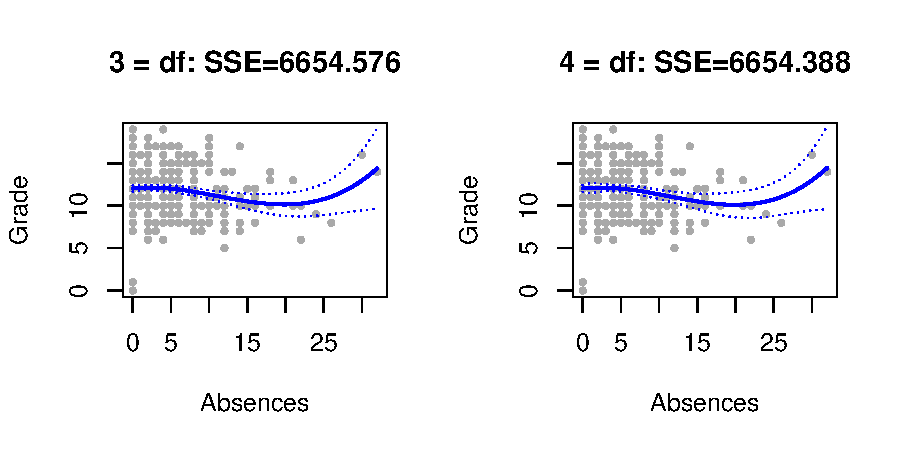
\includegraphics{Report_4-009}

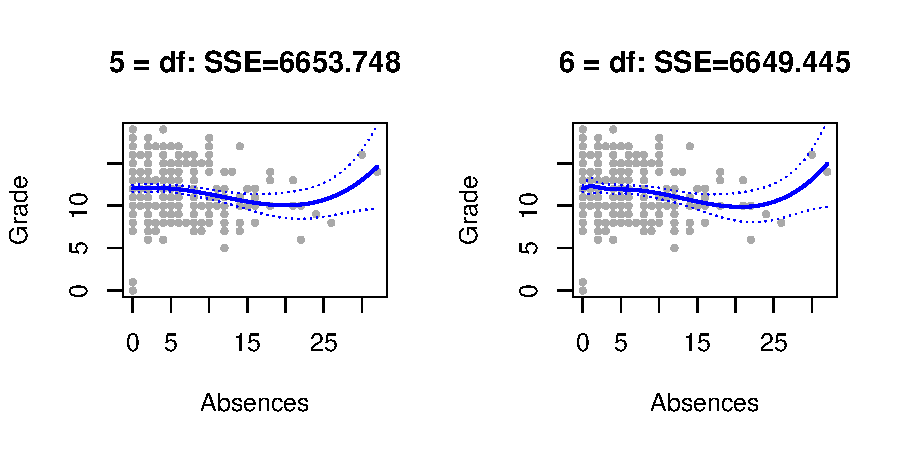
\includegraphics{Report_4-010}

And now onward to LOESS.

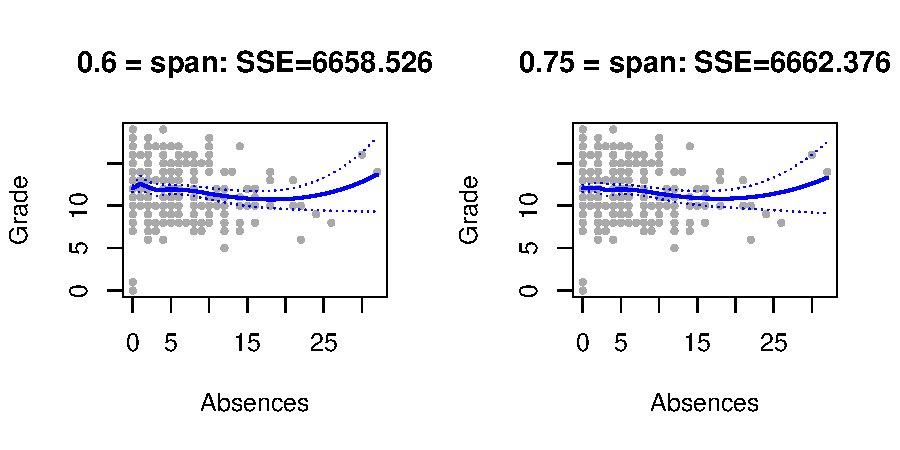
\includegraphics{Report_4-011}

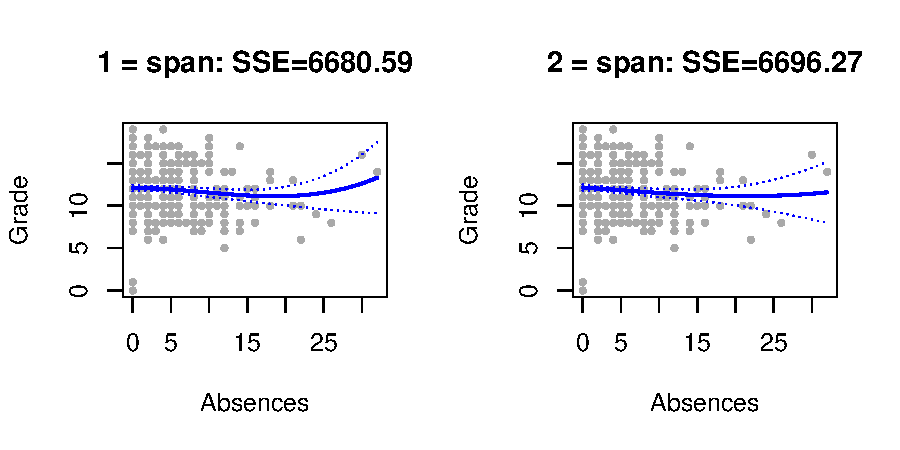
\includegraphics{Report_4-012}

Without cross validating, we would choose the best model. Here's why.
Now to summarize our results for this section. In it, we will comment on anything of interest that occurred. Did anything surprise us? 

\section{Task 2 - Something New}

\subsection{Principal Components Regression}

Next, we perform pricipal components regression on our data. Principal components regression is a dimension-reduction technique for regression. Instead of regressing on $p$ predictors, we regress on $M$ principal components, where principal components are linear combinations of the predictors, and ideally $M<<p$. The first part of PCR is principle component analysis, where, through an iterative process, the principle components are found. This process is as follows: 

\begin{enumerate}
\item Principal component 1 is computed by finding the direction in which the observations vary the most. This is equivalent to finding the line whose distance is shortest to all the observations. 
\item Principal component 2 is computed by finding the line that is orthogonal to principal component 1 and that points in the direction in which the observations on this orthogonal plane now vary the most. 
\item Iterate as in step (2) until you've found $p$ principal components. 
\end{enumerate}

The second part of PCR is to perform a linear regression on the principal components that capture most of your variability. OLS obtains estimates for $\beta_j$ in $$y_i = \beta_0 + \sum \beta_jx_{ij} + \epsilon_i$$ that minimize $$SSE = \sum_{i=1}^{n}\left(Y_i - b_0 - \sum_{j=1}^{p-1}b_jX_{ij}\right)^2$$. On the other hand, PCR obtains estimates for $\beta_j^\prime$ in $$y_i = \beta_0^\prime + \sum_{j=1}^{p\prime}\beta_j^\prime \alpha_{ij} + \epsilon_i$$ that minimize $$SSE = \sum_{i=1}^{n}\left(Y_i - b_0^\prime - \sum_{j=1}^{M-1}b_j^\prime \alpha_{ij}\right)^2$$.

The number of principal components is typically chosen through CV and standardize the predictors before doing PCA ensures that all predictors have equal weight in obtaining the principal components. Otherwise, predictors with higher variance will have a greater impact on the final model.

The idea is that through $M$ principal components, where ideally $M<p$, you can capture most of the variability in the data and the relationship with the response in less dimensions than you would through your $p$ predictors. In this way, PCR also may help prevent overfitting. A key underlying assumption of PCR is that the direction in which the $p$ predictors show the most variation are the directions associated with $Y$. 

PCR is particularly useful for data in which the response can be accurately modeled using only few principal components. We chose PCR because based on our previous models, it seems that most of the variation in our data could potentially be captured in a few components and thus, PCR could give us a more parsimonious model compared to OLS. We also chose it because it could help address any multicolinearity present in our data.

PCR solves issues of multicolinearity, and dimensionality, where the number of observations is less than the number of predictors. 

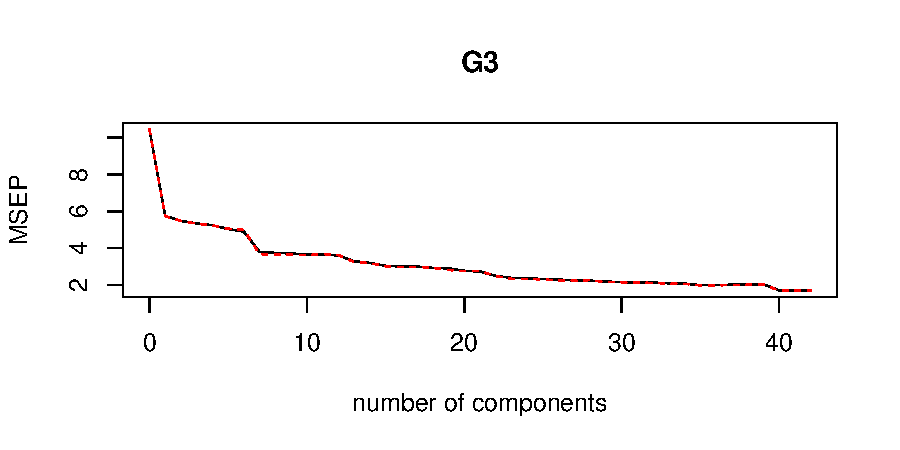
\includegraphics{Report_4-013}


\begin{Schunk}
\begin{Soutput}
[1] 7.878287
\end{Soutput}
\end{Schunk}


We chose to have 7 principal components in our model based on the CV error. The test error for this this number of principal components is 6.92.

\subsection{Inverse Predictions}

Regression models of Y on X can also be used to make an inverse prediction of X on Y. That is, predicting what X might have resulted in the observed Y value. In the context of our data set, we were interested in making inverse predictions of the variable $studytime_num$ - weekly hours studies - based on a student's grades. This might be useful for recommending study time to achieve certain grades. Obtaining inverse predictions is a matter of a simple reformulation of our usual estimated regression model

$$\hat{Y}=b_{0} + b_{1}X$$

to get 

$$\hat{X}_{h(new)} = \frac{Y_{h(new)}-b_{0}}{b_{1}}$$



studytime_num - weekly studytime

\subsection{Added Variable Plots}



\section{Task 3 - Summary}



\end{document}
